\subsection{Superthreshold Operation}

% Above threshold
But what happens now if we increase $V_{gs}$ so that we do not operate in subthreshold anymore? Remember from chapter that free electrons become attracted to the surface of the channel once we operate in superthreshold regime. The electrical charge at the surface consequently starts to increase. This charge is called the inversion charge $Q_i$. Any changes in the gate charge $Q_g$, caused by a change in the gate voltage $V_g$, is now balanced by changes in the inversion charge $Q_i$.\\

\begin{equation}
    Q_g = Q_d + Q_i
\end{equation}\\

where $Q_d$ is the charge of the depletion region. In subthreshold, there is no inversion charge and changes in $Q_g$ are solely balanced by changes in the depletion charge. Remember that $Q_d = C_{dep} \Delta \Psi_s$, so $Q_g$ is mainly counterbalanced by changes in the surface potential $\Psi_s$. The inversion charge $Q_i$ is defined by the following equation:\\

\begin{equation}
    Q_i = C_{ox} (V_g - V_T) = C_{ox} V_{ov}
\end{equation}\\

where $V_T$ is the threshold voltage. The inversion charge $Q_i$ hence simply represents the additional charge that is accumulated once we enter the superthreshold regime. The difference between the gate voltage $V_g$ and the threshold voltage $V_T$ is called the overdrive voltage $V_{ov}$. Figure \ref{fig:vg_vs_qi} demonstrates the relationship between $V_g$ and the inversion charge $Q_i$ as well as the surface potential $\Psi_s$.\\

\begin{figure}
    \centering
    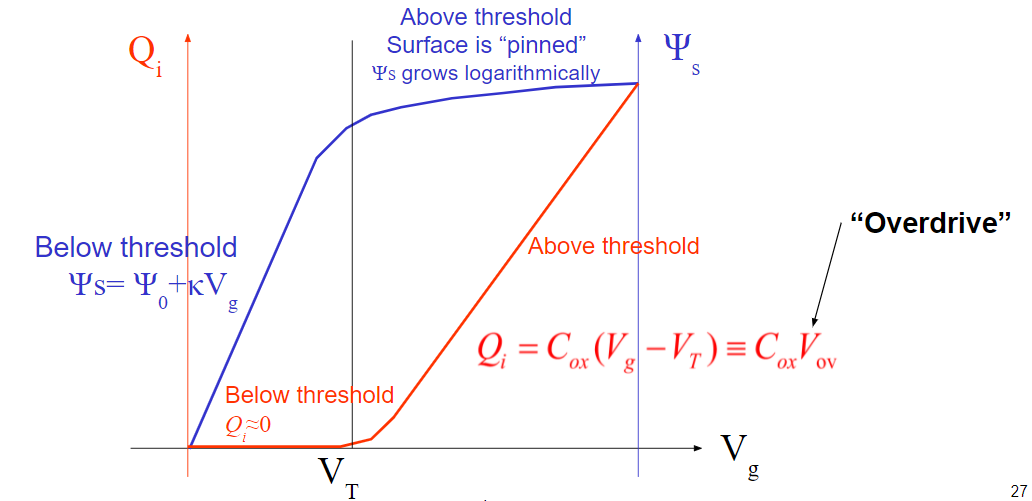
\includegraphics[width=\linewidth]{Figures/Vg_vs_Qi.PNG}
    \caption{Relationship between the gate voltage $V_g$ and the inversion charge $Q_i$ as well as the surface potential $\Psi_s$.}
    \label{fig:vg_vs_qi}
\end{figure}

Remember that in superthreshold the current is generated by an electrical field $I_{ds} = qN \mu \xi$. With $N$ being the number of free carriers and $q$ the electron charge, the product $qN$ simply corresponds to the inversion charge at the surface of the channel along the width of the transistor. The electron field $\xi$ is defined as the potential difference along the field divided by its length.\\

\begin{equation}
    qN = Q_i W = C_{ox} (V_{gs} - V_T) W
\end{equation}

\begin{equation}
    \xi = \frac{V}{d} = \frac{V_{ds}}{L}
\end{equation}

\begin{equation}
    I_{ds} = qN \mu \xi = \mu C_{ox} \frac{W}{L} (V_{gs} - V_T) V_{ds} = \beta (V_{gs} - V_T) V_{ds}
\end{equation}\\

with $\beta = \mu C_{ox} \frac{W}{L}$.